\section{ttbb}
\label{sec:ttbb}

\subsection{Samples}
Four Monte Carlo (MC) generators are compared in this study. % , where the inclusive $\mathrm{t\bar{t}}$ PP8 sample was previously used as the nominal background estimate in the ttH analysis. 
One sample is generated with the \textsc{POWHEG-BOX v2} NLO event generator~\cite{Nason:2004rx,Frixione:2007vw,Alioli:2010xd,Campbell:2014kua} with NNPDF3.0 NLO PDF set, matched to Pythia8 and is referred to as PP8 $\mathrm{t\bar{t}}$, where the additional bb-pair is described by the parton shower. The $h_{damp}$ parameter was set to 1.5 times the top quark mass~\cite{ATL-PHYS-PUB-2016-020}, which is assumed to be 172.5~GeV. The parton shower and the hadronisation were modelled by Pythia 8.210~\cite{PhysRevD.78.014026} with the A14 set of tuned parameters~\cite{ATL-PHYS-PUB-2014-021}. The renormalisation and factorisation scales were set to the transverse mass of the top quark, defined as $m_{T,t} = \sqrt{m^2_t + p^2_{T,t}}$, where $p_{T,t}$ is the transverse momentum of the top quark in the $t\overline{t}$ center-of-mass reference frame. This sample was previously used as the nominal background estimate in the ttH(bb) analysis.
The intrinsic uncertainty of the nominal PP8 $\mathrm{t\bar{t}}$ sample is expressed by the simultaneous variation of the renormalisation and factorisation scales ($\mu_R$ and $\mu_F$) together with the corresponding A14 Eigentune variation parameters. The RadiationUp variation has the renormalisation and factorisation scales decreased by a factor of two, the Var3c upward variation of the A14 parameter set and the $h_{damp}$ parameter doubled. The RadiationDown variation has the renormalisation and factorisation scales increased by a factor of two, the Var3c downward variation and the nominal value of $h_{damp}$.
Additionally, the up and down radiation uncertainty is calculated following the CMS approach, under which the renormalisation scale, factorisation scale and PDF tune variations are each taken individually and their difference to the nominal is summed in quadrature, without changing $h_{damp}$.

The PP8 $\mathrm{t\bar{t}b\bar{b}}$ sample also uses the POWHEG generator where $t\bar{t}+b\bar{b}$ matrix elements are calculated at NLO with massive b-quarks, using the four-flavour NNPDF30 NLO as 0118 4FS PDF set~\cite{Jezo:2018yaf}. The parton shower and hadronisation is modelled by Pythia 8.240. The scales are set to $\mu_R=\sqrt[4]{m_{T,t}\times m_{T,\bar{t}}\times m_{T,b}\times m_{T,\bar{b}} }$, $\mu_F=0.5\times(m_{T,t}+m_{T,\bar{t}}+m_{T,b}+ m_{T,\bar{b}}+m_{T,gluon})$ and $h_{damp}=H_T/2$.

For the PP8 samples the bottom and charm quark decays are described by \textsc{EVTGEN} v1.2~\cite{LANGE2001152} and the top quark spin correlations follow ref.~\cite{Frixione:2007zp}.

The \textsc{Sherpa} $\mathrm{t\bar{t}b\bar{b}}$ sample was generated using \textsc{Sherpa}-\textsc{Openloops}~\cite{Cascioli:2013era}. The $t\bar{t}b\bar{b}$ matrix elements were calculated with massive b-quarks at NLO, using the \textsc{COMIX}~\cite{gleisberg2008comix} and \textsc{OPENLOOPS}~\cite{Cascioli:2011va} matrix element generators, and merged with the Sherpa parton shower, tuned by the authors~\cite{schumann2007parton}. The four-flavour NNPDF30 NNLO as 0118 4FS PDF set was used. The scales are set to $\mu_R=\sqrt[4]{m_{T,t}\times m_{T,\bar{t}}\times m_{T,b}\times m_{T,\bar{b}}}$ and $\mu_F=\sqrt{\Sigma(E_T)}$ over all final state particles.

Both the PP8 $\mathrm{t\bar{t}b\bar{b}}$ and the \textsc{Sherpa} $\mathrm{t\bar{t}b\bar{b}}$ samples describe the additional bb-pair with NLO precision in QCD, taking into account the b-quark mass.

The \textsc{Sherpa} $\mathrm{t\bar{t}}$ sample uses \textsc{Sherpa} version 2.2.1~\cite{Gleisberg:2008ta} with the \textsc{MEPS}@NLO (multi-leg) setup using the \textsc{MEPS}@NLO prescription~\cite{Hoeche:2012yf}, interfaced with \textsc{Openloops}. It provides NLO accuracy for up to one additional parton and LO accuracy for up to four additional partons. The NNPDF3.0 NNLO PDF set is used with a five-flavour scheme and both renormalisation and factorisation scales are set to $\sqrt{0.5\times(m_{T,t}^2+m_{T,\bar{t}}^2)}$. 
A summary of all samples used is given in Table~\ref{tab:ttbbsamples}. All samples are filtered to contain only semi-leptonic $\mathrm{t\bar{t}}$ decays.

\begin{table}
\begin{center}
\caption{\label{tab:ttbbsamples}
The configurations used for the event generation of ttbb processes.}
\vspace{0.25cm}
{\small
\setlength\tabcolsep{1.5pt}
\begin{tabular}{llllll}
\hline\hline
Process & Generator & ME order & Parton shower & PDF & Tune  \\
%& (alternative) & (alternative) & & \\
\hline
$\ttbar$  & \textsc{PowHeg v2} & \textsc{NLO} & \textsc{Pythia 8} &  5FS NNPDF3.0 NLO & \textsc{A14}  \\
$\ttbar+b\bar{b}$  & \textsc{PowHeg v2} & \textsc{NLO} & \textsc{Pythia 8} &  4FS NNPDF30 NLO as 0118& \textsc{A14}  \\
$\ttbar+b\bar{b}$  & \textsc{Sherpa 2.2.1} & \textsc{NLO} & \textsc{Sherpa} &  4FS NNPDF30 NNLO as 0118 & \textsc{Sherpa} default  \\
$\ttbar$  & \textsc{Sherpa 2.2.1} & tt+0,1\@NLO+2,3,4@LO & \textsc{Sherpa} &  5FS NNPDF3.0 NNLO & \textsc{Sherpa} default  \\
\hline\hline
\end{tabular}
}
\end{center}
\end{table}

\subsection{Fiducial Volume}
Object and event selection is defined at particle-level that closely matches the detector-level described in reference~\cite{HIGG-2017-03} and was defined together with CMS as a common phase space. Jets are reconstructed from stable particles with a mean lifetime of $\tau > 3\times 10^{-11}$~s, using the anti-$k_t$ algorithm with a radius parameter of $R=0.4$, and are required to have transverse momentum $p_{T}>25~\GeV$ and pseudorapidity $|\eta|< 2.5$. Jets that are matched to b-hadrons with $p_{T}>5~\GeV$ by ghost matching~\cite{Cacciari:2008gn} and are referred to as b-jets. Electrons and muons, referred to as leptons, are required to satisfy $p_{T}>27~\GeV$ and $|\eta|< 2.5$. 
Leptons are removed if they are separated from a jet by less than $\Delta R>0.4$ ($\Delta R = \sqrt{(\Delta \eta )^2 + (\Delta \phi)^2}$).
%Selected leptons are required to be separated from selected jets by $\Delta R>0.4$. 
Events are selected with exactly one lepton and at least 4 jets, equivalent to the semi-leptonic $\mathrm{t\bar{t}}$ decay.
%Two regions are considered, defined by 3 b-jets or $\geq$4 b-jets.
Two analysis regions are considered. The first is defined by the presence of exactly three selected $b$-jets (3b selection), while the second requires four or more such $b$-jets (4b selection).


%, , , , , , $N_{jets}$, 
\begin{table}[]
\begin{center}
\caption{\label{tab:ttbb_varlist}
The list of the validation variables for the comparison of the generators for $ttbb$ process.}
\vspace{0.25cm}
{\small
\setlength\tabcolsep{1.5pt}
\begin{tabular}{l|l}
\hline\hline
Variable & Description  \\ \hline
average $\Delta R (b,b)$&    average over $\Delta R(b, b)$ build from all 2 b-jet combinations in the event           \\ 
min $\Delta R (b,b)$ &    $\Delta R$ of the two b-jets in the event which are closest in $\Delta R $          \\ 
$M (b,b)_{maxP_T}$ &      mass of the 2 b-jet system build of the b-jets with maximal $p_T$         \\ 
$M (b,b)_{min\Delta R(b,b)}$ &         mass of the 2 b-jet system build of the b-jets closest in $\Delta R $     \\ 
$H_T$  $b$-jets&           scalar sum of all b-jet $p_T$ in the event    \\ 
$H_T$ light-jets&        scalar sum of $p_T$ of all light jets in the event       \\ 
$N_{jets}$   &     number of all jets in the event (including b-jets)          \\ 
jet eta &          $\eta$ of any jet in the event     \\ 
    \hline\hline    
\end{tabular}
}
\end{center}
\end{table}




\subsection{Results}
The nominal PP8 $\mathrm{t\bar{t}}$ sample and the alternative generators are normalised to an integral of 1, after all cuts and in each histogram individually for a shape-only comparison.
The radiation uncertainty variations on PP8 $\mathrm{t\bar{t}}$ are added and include normalisation differences with respect to the central value. For the RadiationUp uncertainty, an alternative sample with different $h_{damp}$ was used, here the number of events (not the sum of weights) was scaled to the central value.
The central value of the PP8 $\mathrm{t\bar{t}}$ and the other three generators are normalised to 1. The first ratio plot shows the ratio of the different MC samples to PP8 $\mathrm{t\bar{t}}$ from the upper plot, where the colour scheme is given in the legend.
The list of the validation variables for this comparison is presented in this note summarised in Table~\ref{tab:ttbb_varlist}.

Discrepancies between PP8 $\mathrm{t\bar{t}}$ and the alternative generators can be seen in the $\Delta R$ quantities, as in Figures~\ref{ttbb:avedR} and \ref{ttbb:mindR}, where at least in the 4b selection the difference to the alternative generators is larger than the uncertainty band given by the radiation variations.  
%In the b-jet pair invariant mass variables $\mathrm{M_{bb}^{max P_T}}$ and $\mathrm{M_{bb}^{min \Delta R}}$ shown in Figures~\ref{ttbb:MbbmaxPT} and~\ref{ttbb:MbbminDR}, the largest difference is seen between the Sherpa $\mathrm{t\bar{t}}$ and all other samples.
Two types of $b$-jet pairs are defined: one pair is build from the two $b$-jets with the highest $p_T$ sum, called $maxP_T$, and one pair from the two $b$-jets which are closest in $\Delta R$, called $min \Delta R$ . The invariant mass of the b-jet pairs are shown in Figures~\ref{ttbb:MbbmaxPT} and~\ref{ttbb:MbbminDR}, the largest difference is seen between the Sherpa $\mathrm{t\bar{t}}$ and all other samples.
%
Differences are also observed in the $\mathrm{H_T}$ distributions, particularly in the 3b selection. In $\mathrm{H_T}$ of all b-jets, as in Figures~\ref{ttbb:HTbjets}, one observes a difference between PP8 $\mathrm{t\bar{t}}$ and the samples with b-jets in the matrix element, while in $\mathrm{H_T}$ of all light jets, shown in Figure~\ref{ttbb:HTljets}, a difference between the 4 and 5 flavour schemes can be seen. The jet multiplicity, as in Figure~\ref{ttbb:Njets}, has poor agreement among the generators for large jet multiplicities.
Lastly, differences among the samples are shown for the $\mathrm{\eta_{jet}}$ distribution, in Figure~\ref{ttbb:jeteta}.

The second ratio plot shows the relative uncertainty of the radiation variations on PP8 $\mathrm{t\bar{t}}$, shown as the ratio of the varied sample to the nominal for two cases described above, where the scale and A14 Eigentune parameters are either varied simultaneously (black) or individually and then summed following the CMS approach (red). $h_{damp}$ variations are only considered for the first case.



\begin{figure}[!htb]
\centering
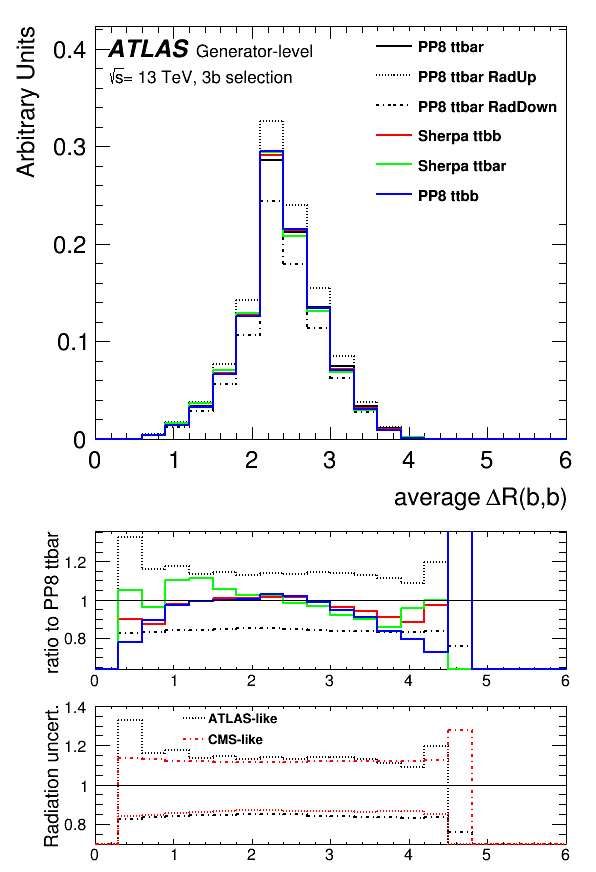
\includegraphics[width=0.38\textwidth]{Plots/ttbb/hisgenEvt_Dr_GenBJetsAverage_4j3t__div}
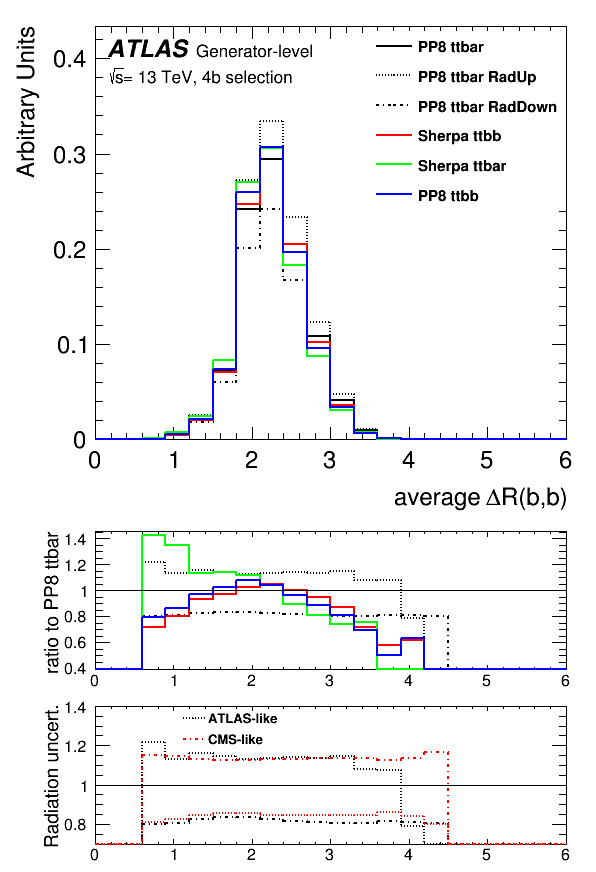
\includegraphics[width=0.38\textwidth]{Plots/ttbb/hisgenEvt_Dr_GenBJetsAverage_4j4t__div}
  \caption{Distribution of the average opening angle between two b-jets, for the 3b selection (left) and the 4b-jet selection (right). The central value of the PP8 $\mathrm{t\bar{t}}$ and the other three generators are normalised to 1. The first ratio shows the different curves divided by PP8 $\mathrm{t\bar{t}}$. The second ratio plot shows the relative uncertainty of the radiation variations divided by the nominal PP8 $\mathrm{t\bar{t}}$ following the above description of simultaneous variations (black) and as the sum of individual variations following the CMS approach (red).  \label{ttbb:avedR}}
\end{figure}

\begin{figure}[!htb]
\centering
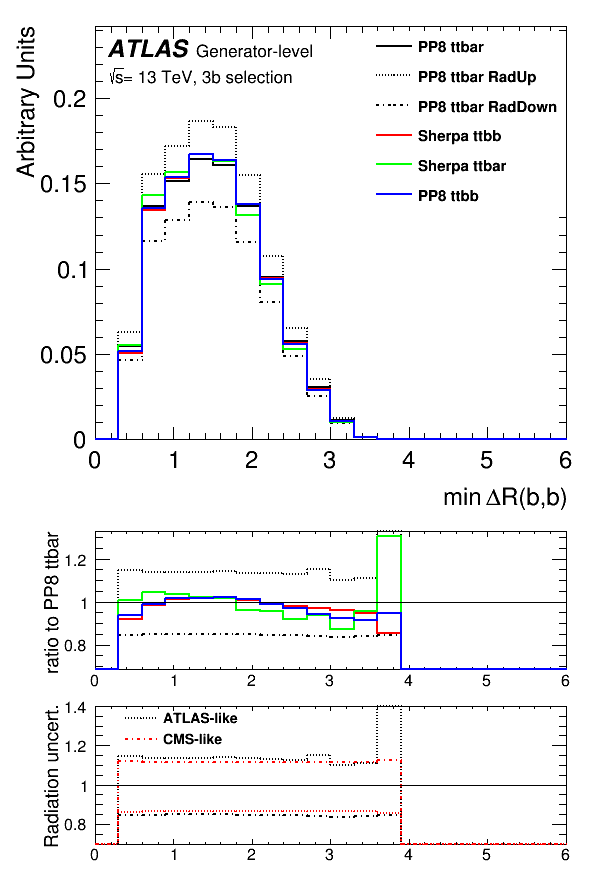
\includegraphics[width=0.38\textwidth]{Plots/ttbb/hisgenEvt_Dr_MinDeltaRGenBJets_4j3t__div}
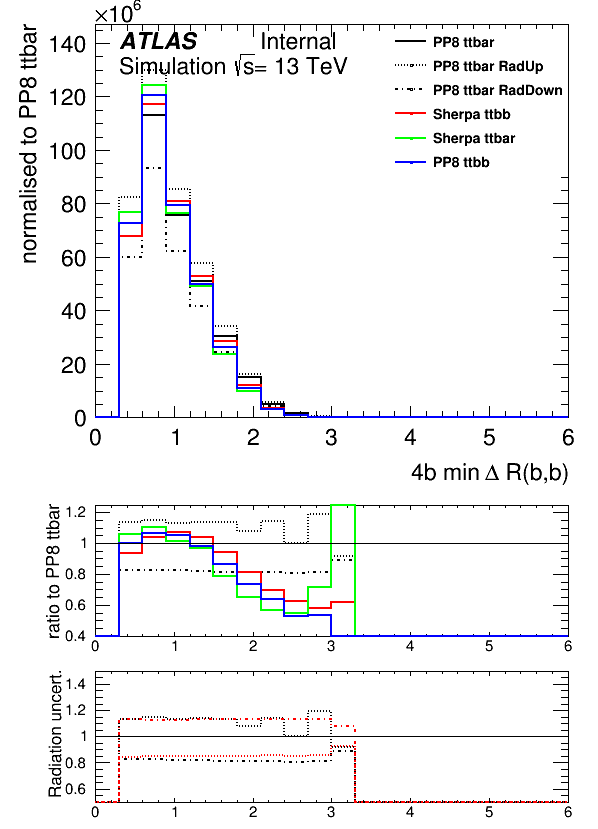
\includegraphics[width=0.38\textwidth]{Plots/ttbb/hisgenEvt_Dr_MinDeltaRGenBJets_4j4t__div}
  \caption{Distribution of the smallest opening angle between two b-jets, for the 3b selection (left) and the 4b-jet selection (right). The central value of the PP8 $\mathrm{t\bar{t}}$ and the other three generators are normalised to 1. The first ratio shows the different curves divided by PP8 $\mathrm{t\bar{t}}$. The second ratio plot shows the relative uncertainty of the radiation variations divided by the nominal PP8 $\mathrm{t\bar{t}}$ following the above description of simultaneous variations (black) and as the sum of individual variations following the CMS approach (red). \label{ttbb:mindR}}
\end{figure}

\begin{figure}[!htb]
\centering
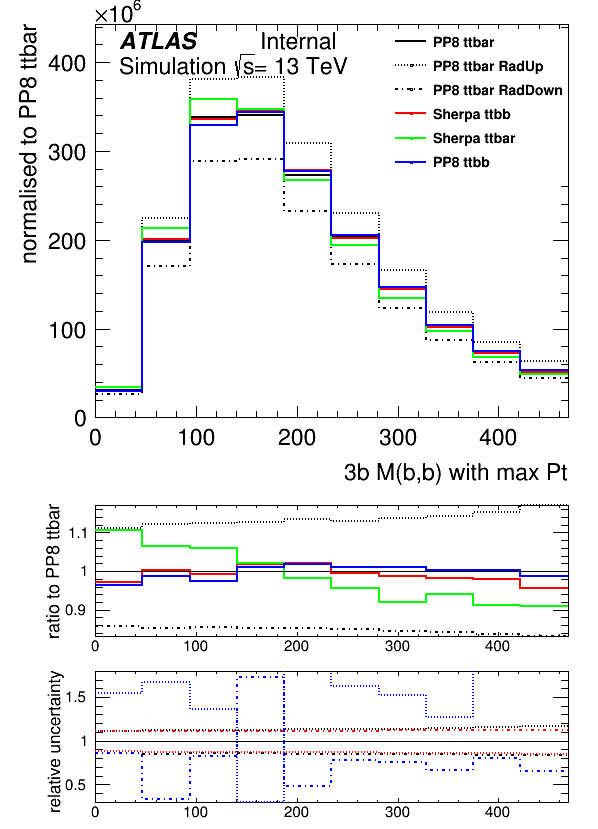
\includegraphics[width=0.38\textwidth]{Plots/ttbb/hisgenEvt_M_HardestGenBJets_4j3t__div}
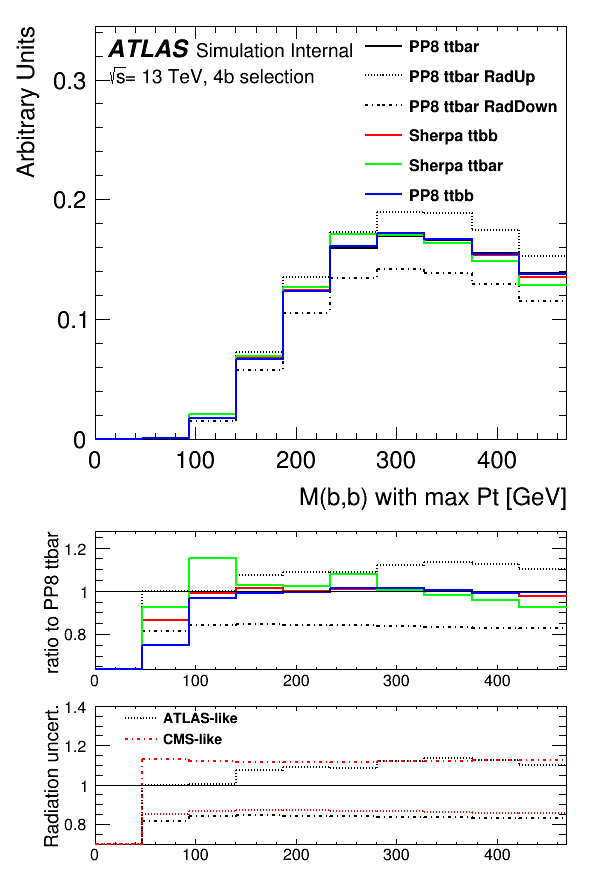
\includegraphics[width=0.38\textwidth]{Plots/ttbb/hisgenEvt_M_HardestGenBJets_4j4t__div}
  \caption{Distribution of the invariant mass in GeV of the two b-jets with the highest $\mathrm{P_T}$ sum, for the 3b selection (left) and the 4b-jet selection (right). The central value of the PP8 $\mathrm{t\bar{t}}$ and the other three generators are normalised to 1. The first ratio shows the different curves divided by PP8 $\mathrm{t\bar{t}}$. The second ratio plot shows the relative uncertainty of the radiation variations divided by the nominal PP8 $\mathrm{t\bar{t}}$ following the above description of simultaneous variations (black) and as the sum of individual variations following the CMS approach (red). \label{ttbb:MbbmaxPT}}
\end{figure}

\begin{figure}[!htb]
\centering
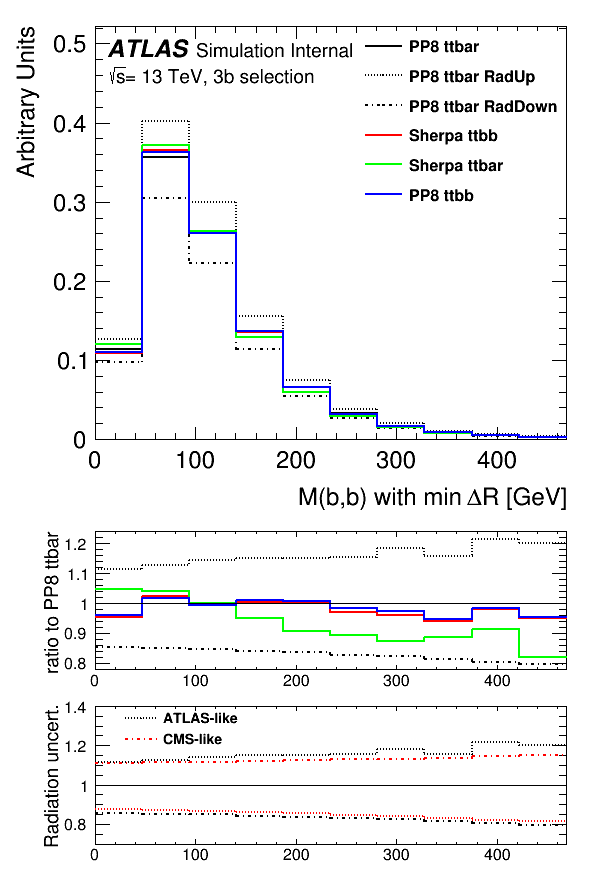
\includegraphics[width=0.38\textwidth]{Plots/ttbb/hisgenEvt_M_MinDeltaRGenBJets_4j3t__div}
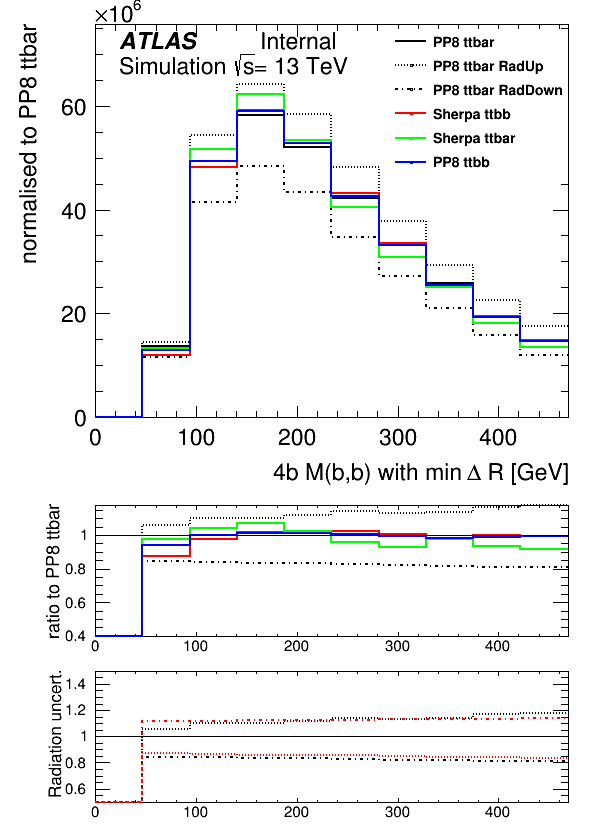
\includegraphics[width=0.38\textwidth]{Plots/ttbb/hisgenEvt_M_MinDeltaRGenBJets_4j4t__div}
  \caption{Distribution of the invariant mass in GeV of the two b-jets with the smallest opening angle, for the 3b selection (left) and the 4b-jet selection (right). The central value of the PP8 $\mathrm{t\bar{t}}$ and the other three generators are normalised to 1. The first ratio shows the different curves divided by PP8 $\mathrm{t\bar{t}}$. The second ratio plot shows the relative uncertainty of the radiation variations divided by the nominal PP8 $\mathrm{t\bar{t}}$ following the above description of simultaneous variations (black) and as the sum of individual variations following the CMS approach (red). \label{ttbb:MbbminDR}}
\end{figure}

\begin{figure}[!htb]
\centering
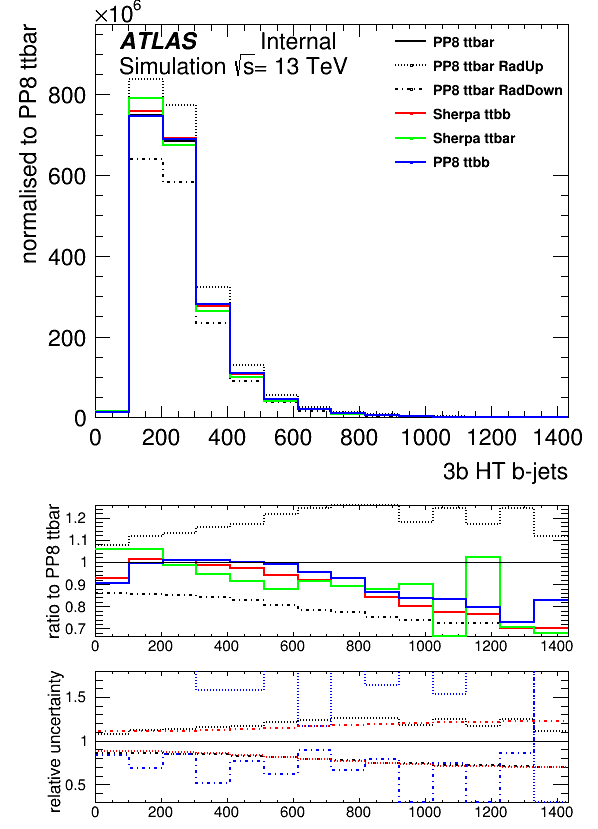
\includegraphics[width=0.38\textwidth]{Plots/ttbb/hisgenHTbjets_4j3t__div}
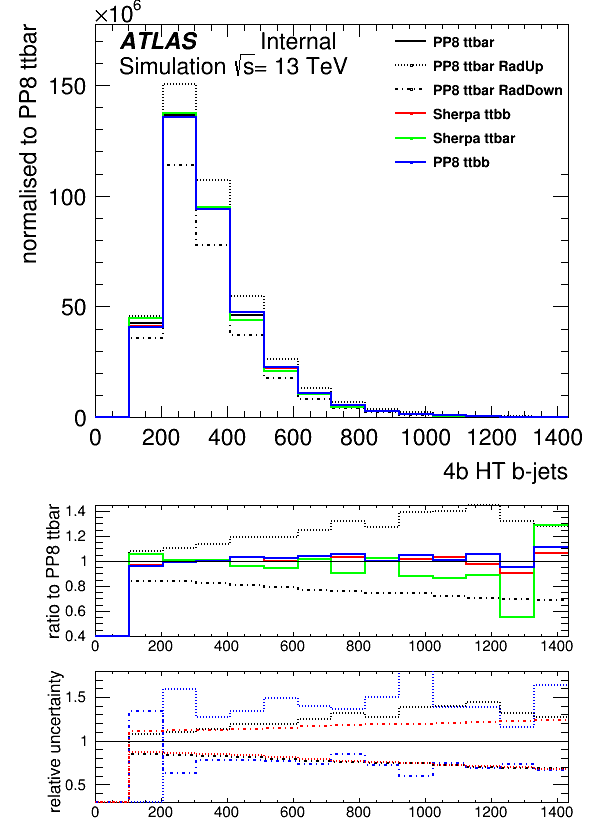
\includegraphics[width=0.38\textwidth]{Plots/ttbb/hisgenHTbjets_4j4t__div}
  \caption{Sum of b-jet transverse momenta in GeV, for the 3b selection (left) and the 4b-jet selection (right). The central value of the PP8 $\mathrm{t\bar{t}}$ and the other three generators are normalised to 1. The first ratio shows the different curves divided by PP8 $\mathrm{t\bar{t}}$. The second ratio plot shows the relative uncertainty of the radiation variations divided by the nominal PP8 $\mathrm{t\bar{t}}$ following the above description of simultaneous variations (black) and as the sum of individual variations following the CMS approach (red). \label{ttbb:HTbjets}}
\end{figure}

\begin{figure}[!htb]
\centering
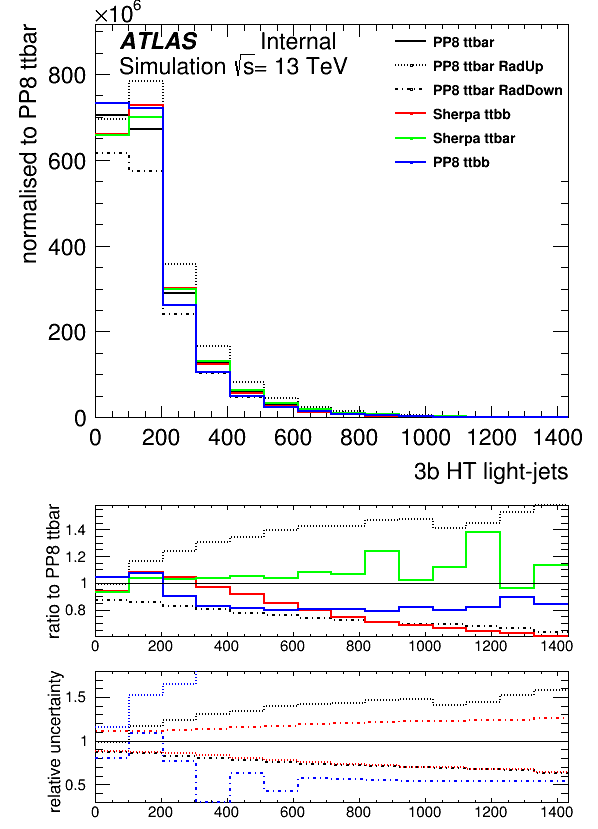
\includegraphics[width=0.38\textwidth]{Plots/ttbb/hisgenHTljets_4j3t__div}
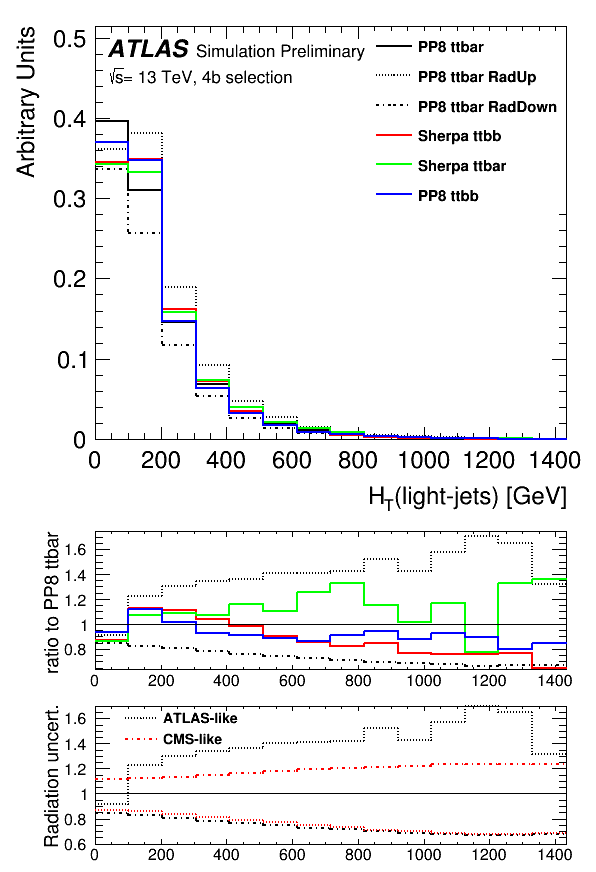
\includegraphics[width=0.38\textwidth]{Plots/ttbb/hisgenHTljets_4j4t__div}
  \caption{Sum of non-b-jet transverse momenta in GeV, for the 3b selection (left) and the 4b-jet selection (right). The central value of the PP8 $\mathrm{t\bar{t}}$ and the other three generators are normalised to 1. The first ratio shows the different curves divided by PP8 $\mathrm{t\bar{t}}$. The second ratio plot shows the relative uncertainty of the radiation variations divided by the nominal PP8 $\mathrm{t\bar{t}}$ following the above description of simultaneous variations (black) and as the sum of individual variations following the CMS approach (red). \label{ttbb:HTljets}}
\end{figure}

\begin{figure}[!htb]
\centering
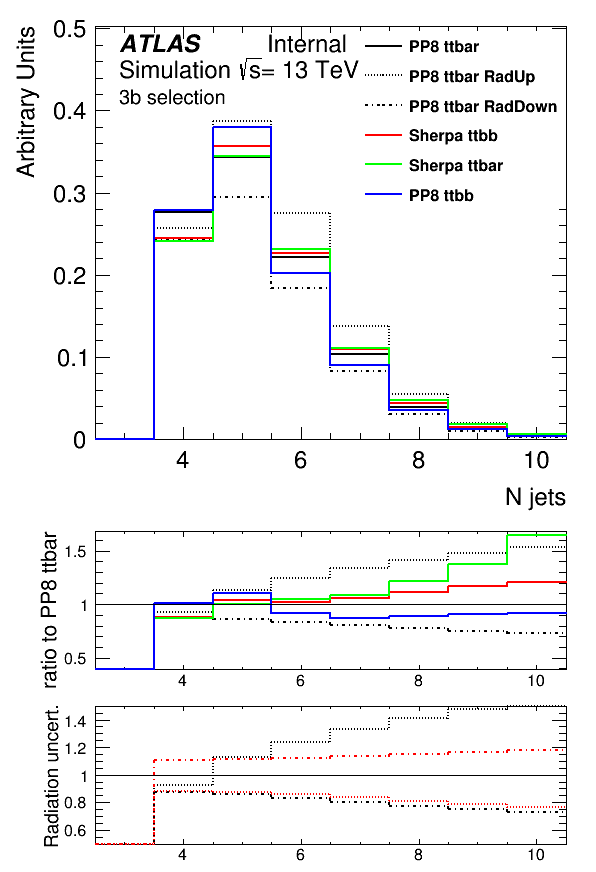
\includegraphics[width=0.38\textwidth]{Plots/ttbb/hisgenNjets_4j3t__div}
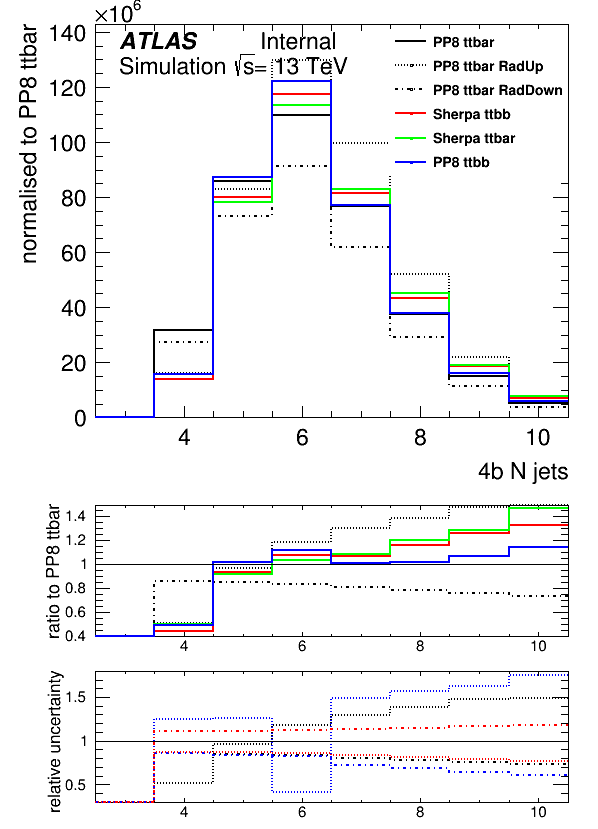
\includegraphics[width=0.38\textwidth]{Plots/ttbb/hisgenNjets_4j4t__div}
  \caption{Jet multiplicity, for the 3b selection (left) and the 4b-jet selection (right). The central value of the PP8 $\mathrm{t\bar{t}}$ and the other three generators are normalised to 1. The first ratio shows the different curves divided by PP8 $\mathrm{t\bar{t}}$. The second ratio plot shows the relative uncertainty of the radiation variations divided by the nominal PP8 $\mathrm{t\bar{t}}$ following the above description of simultaneous variations (black) and as the sum of individual variations following the CMS approach (red). \label{ttbb:Njets}}
\end{figure}

\begin{figure}[!htb]
\centering
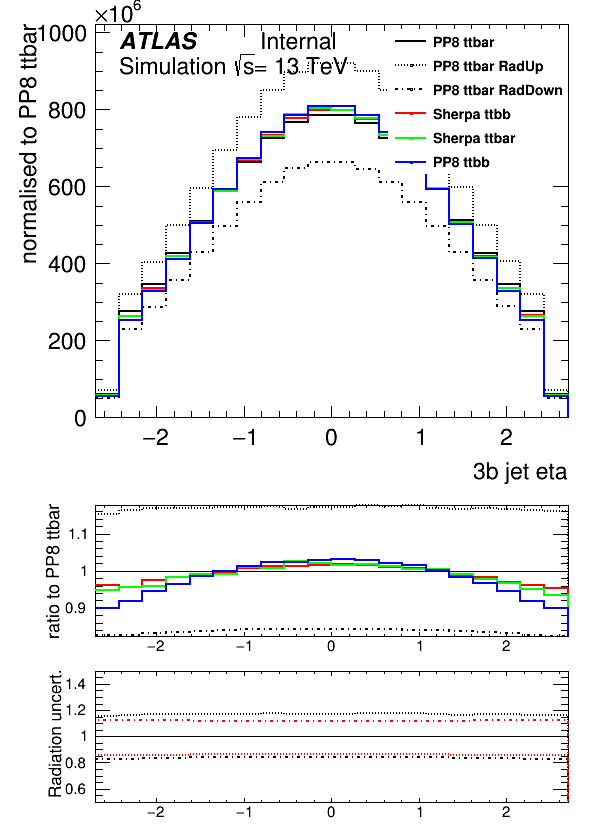
\includegraphics[width=0.38\textwidth]{Plots/ttbb/his3b_jeteta__div}
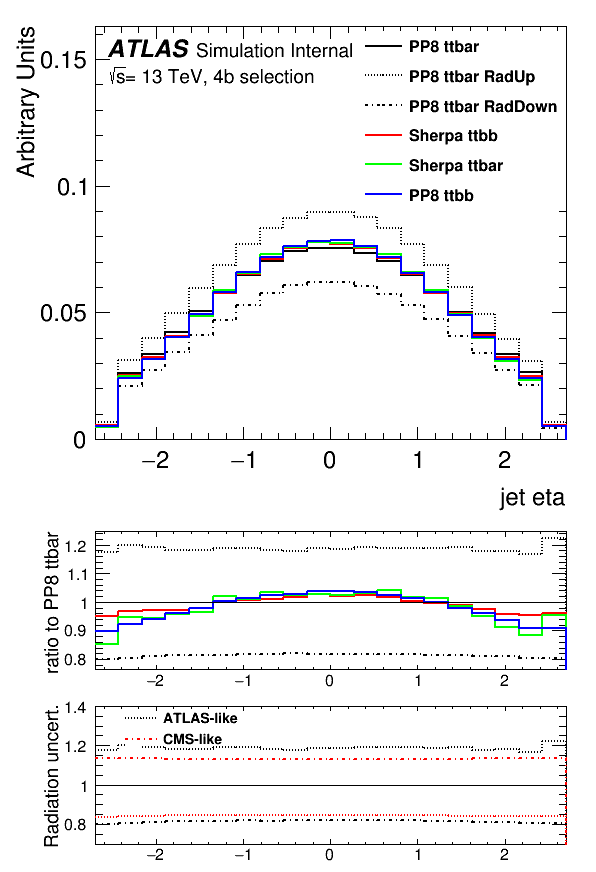
\includegraphics[width=0.38\textwidth]{Plots/ttbb/his4b_jeteta__div}
  \caption{Jet pseudorapidity, for the 3b selection (left) and the 4b-jet selection (right). The central value of the PP8 $\mathrm{t\bar{t}}$ and the other three generators are normalised to 1. The first ratio shows the different curves divided by PP8 $\mathrm{t\bar{t}}$. The second ratio plot shows the relative uncertainty of the radiation variations divided by the nominal PP8 $\mathrm{t\bar{t}}$ following the above description of simultaneous variations (black) and as the sum of individual variations following the CMS approach (red). \label{ttbb:jeteta}}
\end{figure}